\newpage
\section*{Задание 1}
\addcontentsline{toc}{section}{\tocsecindent{Задание 1}}
\large
\subsection*{Постановка задачи}
\begin{figure}[h!]
	\center 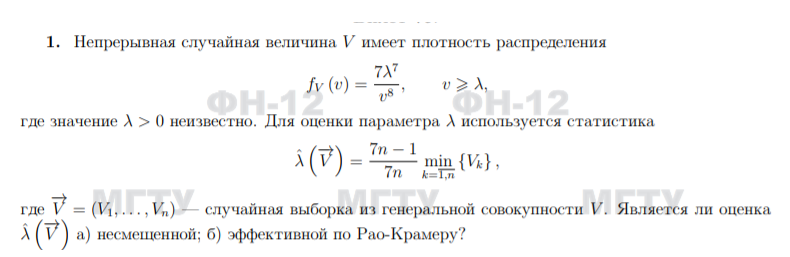
\includegraphics[scale=0.6]{img/us.png}
\end{figure}
\subsection*{Решение}
\begin{figure}[h!]
	\center 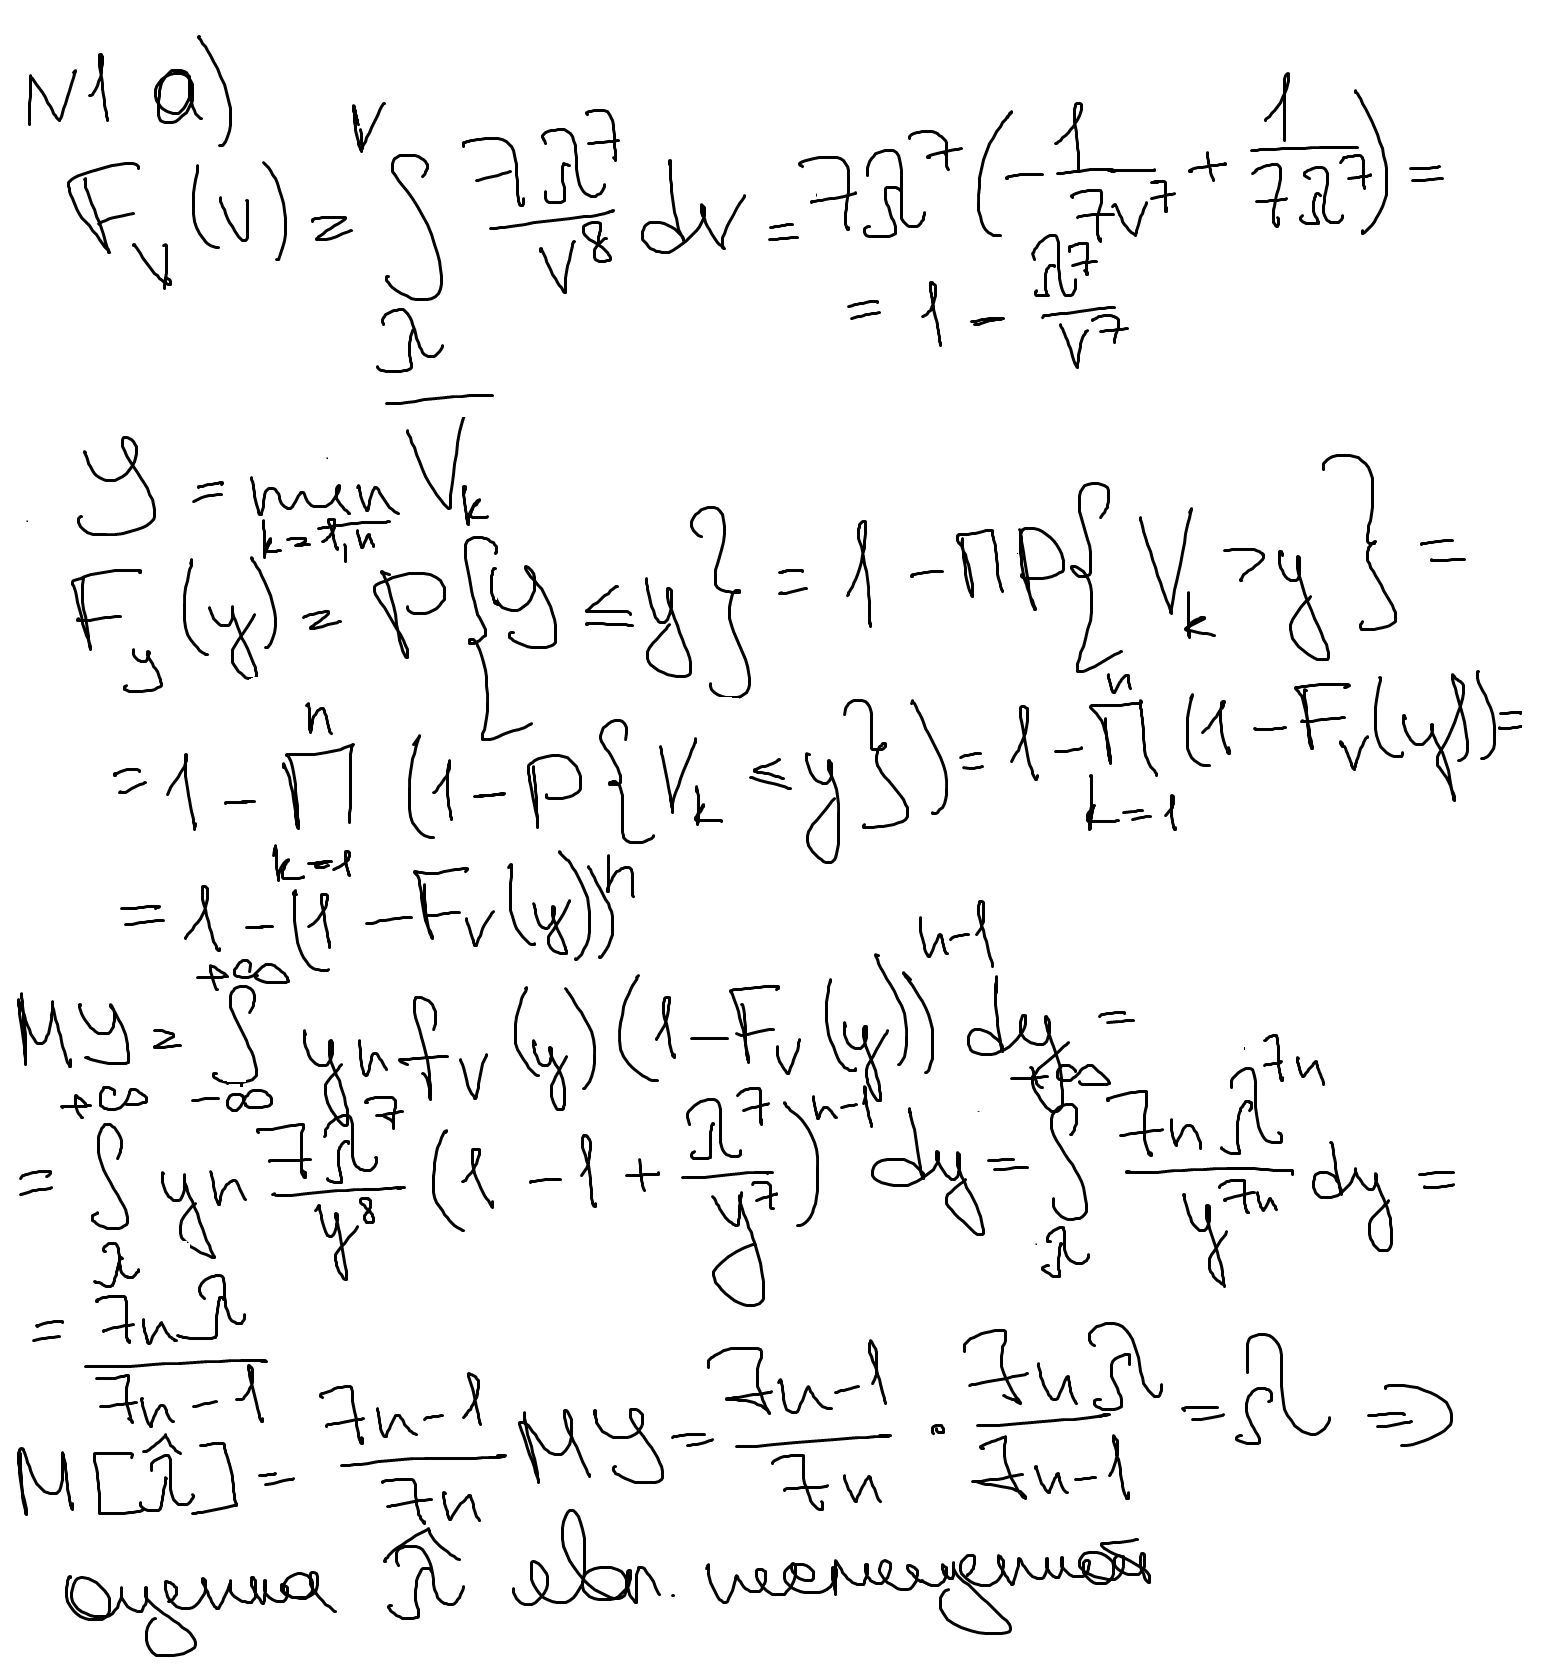
\includegraphics[scale=0.5]{img/resh.png}
\end{figure}
\textbf{Ответ:} а) является несмещенной
\section*{Задание 2}
\addcontentsline{toc}{section}{\tocsecindent{Задание 2}}
\subsection*{Постановка задачи}
Пусть $X \sim Exp (\lambda)$, где значение $\lambda$ неизвестно. Построить для $\lambda$ доверительный интервал
уровня $\gamma $ = 0.8, если после n = 6 испытаний получены значения $\overline{x}=4.32$, $S^2 (\overrightarrow{x}) = 1.69$.
\subsection*{Решение}
Построим доверительный интервал для дисперсии скорости снаряда, используя центральную статистику:
\begin{equation}
T(\vec{X}, \lambda) = 2\lambda n \overline{x} \sim \chi^2(2n)
\end{equation}
Ниже изображен график функции плотности распределения статистики $T$. 
\begin{figure}[h!]
	\caption{График функции плотности распределения статистики $T$}
	\center 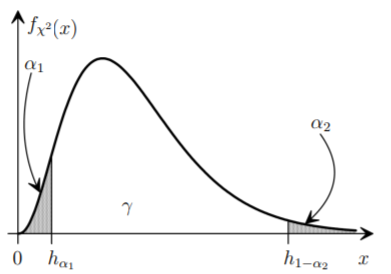
\includegraphics{img/1.png}
\end{figure}\\
В соответствии со свойствами непрерывных случайных величин,
\begin{equation}
\gamma = P\left\{ h_{\frac{1-\alpha}{2}} < T(\vec{X}, \lambda) < h_{\frac{1+\alpha}{2}}\right\}
\end{equation}
Подставим формулу (1) для $T(\vec{X}, \lambda)$:
\begin{equation}
\gamma = P\left\{ h_{0.1} <2\lambda n \overline{x} < h_{0.9}\right\}
\end{equation}
\begin{equation}
\gamma = P\left\{ \frac{h_{0.1}}{2n\overline{x}} < \lambda < \frac{h_{0.9}}{2n\overline{x}}\right\}
\end{equation}
Откуда получим  доверительный интервал уровня $\gamma = 0.8$ для  $\lambda$:
\begin{equation}
0.8 = P\left\{ \frac{6.3}{2\cdot 6 \cdot 4.32} < \lambda <\frac{18.54}{2\cdot 6 \cdot 4.32}\right\}
\end{equation}
\begin{equation}
0.8 = P\left\{ 0.121 < \lambda <0.357\right\}
\end{equation}
\textbf{Ответ:} $\lambda \in (0.121;0.357)$ 